\subsection{Introducción:}

En este ejercicio trabajaremos con todo lo relacionado a la \textit{TSS}, realizaremos los siguientes ítems:

\begin{itemize}



\item [\textit{a)}]  Definir las entradas en la \textit{GDT} que considere necesarias para ser usadas como descriptores de \textit{TSS}.

\item [\textit{b)}] Completar la entrada de la \textit{TSS} de la tarea Idle con la información de la tarea Idle. La tarea Idle se encuentra en la dirección 0x00016000. La pila se alojará en la misma dirección que la pila del kernel y debe compartir el mismo CR3 que el kernel.

\item [\textit{c)}]  Construir una función que complete una TSS libre con los datos correspondientes. El código de las tareas se encuentra a partir de la dirección 0x00010000. Para la dirección de la pila se debe utilizar el mismo espacio de la tarea, la misma crecerá desde la base de la tarea. Para el mapa de memoria se debe construir uno nuevo utilizando la función \textit{mmu\_inicializar\_dir\_perro}. Además, tener en cuenta que cada tarea utilizará una pila distinta de nivel 0. 

\item [\textit{d)}] Completar la entrada de la \textit{GDT} correspondiente a la tarea\_inicial.

\item [\textit{e)}]  Completar la entrada de la \textit{GDT} correspondiente a la tarea Idle.

\item [\textit{f)}]  Escribir el código necesario para ejecutar la tarea Idle, es decir, saltar intercambiando las TSS, entre la tarea\_inicial y la tarea Idle.

\item [\textit{g)}] Modificar la rutina de la interrupción 0x46, para que implemente los servicios según se indica en la sección 4.4, sin desalojar a la tarea que realiza el syscall.

\item [\textit{h)}]  Ejecutar una tarea perro manualmente. Es decir, crearla y saltar a la entrada en la \textit{GDT} de su respectiva TSS.

\end{itemize}

\subsection{Ítem a): Definir entradas de la \textit{GDT} necesarias}
Para este punto definimos 18 nuevas entradas en la \textit{GDT}.\\

Las primeras dos nuevas entradas de la \textit{GDT} corresponden a la \textit{Tarea inicial} y a la tarea \textit{idle} respectivamente. 


\begin{figure}[H]
\begin{center}
\minipage{0.6\textwidth}
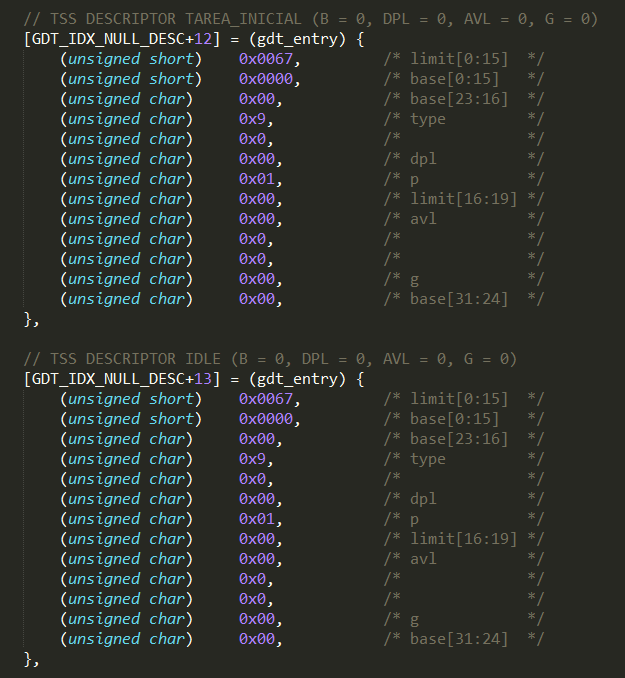
\includegraphics[width=\linewidth]{ejercicio6/gdt_inicial_idle.png}
\caption{{\small \textit{Entrada de la \textit{GDT} correspondiente a la tarea inicial y a la idle }}}
\endminipage
\end{center}
\end{figure}

Las siguientes 8 entradas corresponden a los 8 perros del \textbf{jugador A} ordenadas en orden decreciente en el número de perros, es decir, el \textit{id} y finalmente las últimas 8 entradas corresponden a los 8 perros del \textbf{jugador B } también ordenadas decrecientemente por \textit{id}.\\

\begin{figure}[H]
\begin{center}
\minipage{0.6\textwidth}
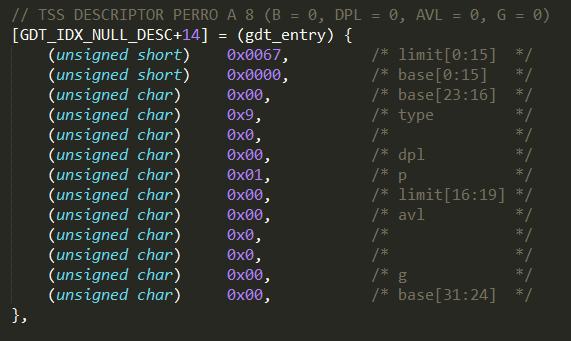
\includegraphics[width=\linewidth]{ejercicio6/gdt_perro.png}
\caption{{\small \textit{Entrada de la \textit{GDT} correspondiente al descriptor de tss de la tarea perro }}}
\endminipage
\end{center}
\end{figure}


\subsection{Ítem b): Completar la $TSS$ de la tarea $idle$ y de la $tarea inicial$}
Para este item hacemos lo siguiente, primero completamos el campo \textit{base} de la entrada de la \textit{GDT} correspondiente a la tarea \textit{idle}.Para ello le asignamos la dirección 0x00016000 tal como indica el enunciado.\\
Como también nos dicen que comparte el \textit{esp} con el \textit{kernel} entonces en la entrada \textit{esp} de la \textit{TSS} le asignamos 0x27000 que era el \textit{esp} asignado al kernel.Además como comparten el \textit{cr3} le asigno a la entrada correspondiente en la \textit{TSS} 0x28000.\\% por qué? ni idea
La siguiente imagen muestra como queda completo el descriptor de la \textit{TSS}\\

\begin{figure}[H]
\begin{center}
\minipage{0.60\textwidth}
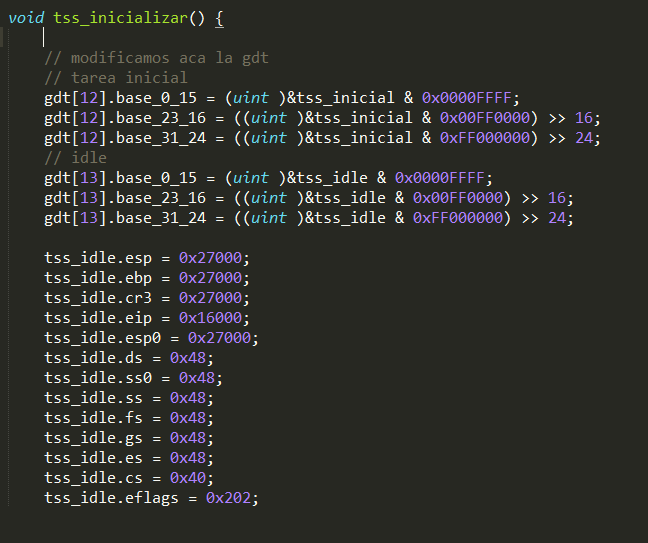
\includegraphics[width=\linewidth]{ejercicio6/tss_iddle_inicial.png}
\caption{{\small \textit{ Completamos el desscriptor de la\textit{TSS} correspondiente a la tarea iddle y a la inicial}}}
\endminipage
\end{center}
\end{figure}



\subsection{Ítem c): Realizar la función $tss\_completar(int$ $jugador, int$ $perro, perro\_t *perro)$}
Lo que nos piden en este punto es hacer la función $void$ $tss\_completar(int$ $jugador, int$ $perro, perro\_t *perro)$\\
Lo primero que  hacemos en esta función es pedir una nueva página libre para usarla como una pila de nivel 0 para la tarea.\\
Lo siguiente es preguntar si es la tarea (el perro) es una tarea correspondiente al \textbf{jugador A} o al \textbf{jugador B}. Para saber donde guardar el descriptor. Para cada perro de ambos jugadores se realiza lo siguiente:
\begin{itemize}

\item En los campos \textit{cs}, \textit{es}, \textit{gs}, \text{ss}, \textit{ds}, \textit{fs} tienen los segmentos definidos anteriormente en la \textit{GDT}.
\item La entrada \textit{esp} tiene 0x0402000-12.
\item La entrada \textit{eip} tiene 0x00401000.
\item La entrada \textit{eflags} = 0x202.
\item La entrada \textit{esp0} = Es la posicion de la página libre pedida mas 4kb pues tiene apilado en la pila los argumentos.
\item La entrada \textit{iomap} = 0xFFFF.
\item La entrada \textit{ss0} = 0x48.
\item El nuevo \textit{cr3} va a ser el devuelto por la función \textit{mmu\_inicializar\_memoria\_perro}. Asignamos el \textit{cr3}  al campo correspondiente y actualizamos la entrada correspondiente a la \textit{GDT} para esa tarea seteando los campos base e índice.
\end{itemize}

La siguiente imágen muestra dicho proceso.\\

\begin{figure}[H]
\begin{center}
\minipage{0.6\textwidth}
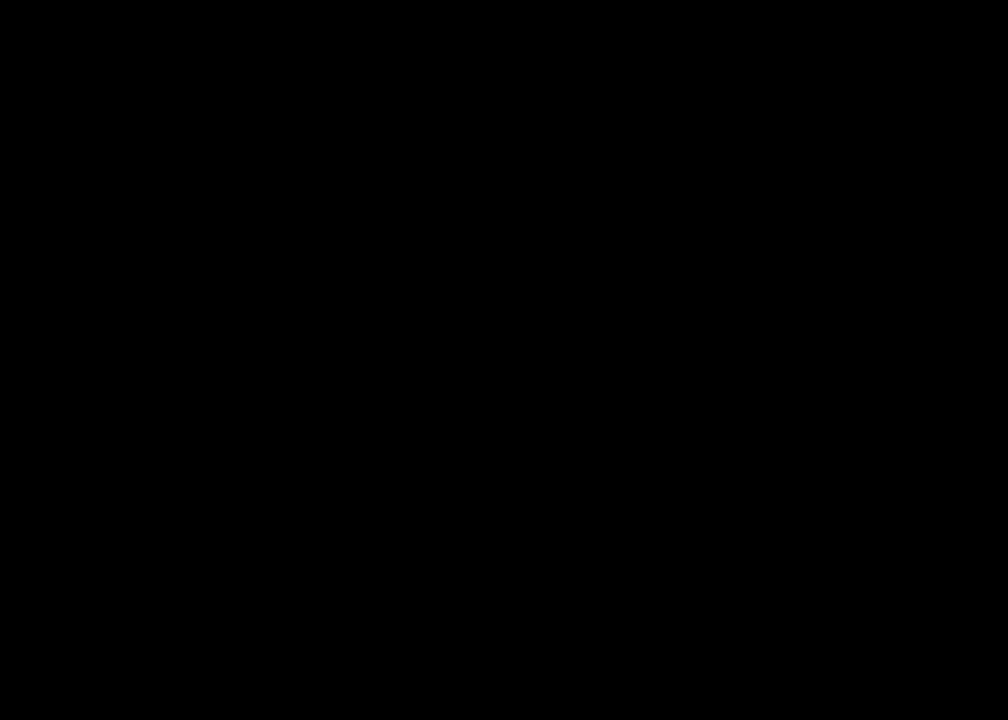
\includegraphics[width=\linewidth]{ejercicio6/tss_perro.png}
\caption{{\small }}
\endminipage
\end{center}
\end{figure}


\subsection{Ítem d): Completar la entrada de la $tarea\_inicial$ en la $GDT$}

La entrada de la \textit{GDT} correspondiente a la tarea inicial en principio la definimos con cualquier valor  en la base pero con los valores correspondientes en los demás campos.

\begin{figure}[H]
\begin{center}
\minipage{1.00\textwidth}
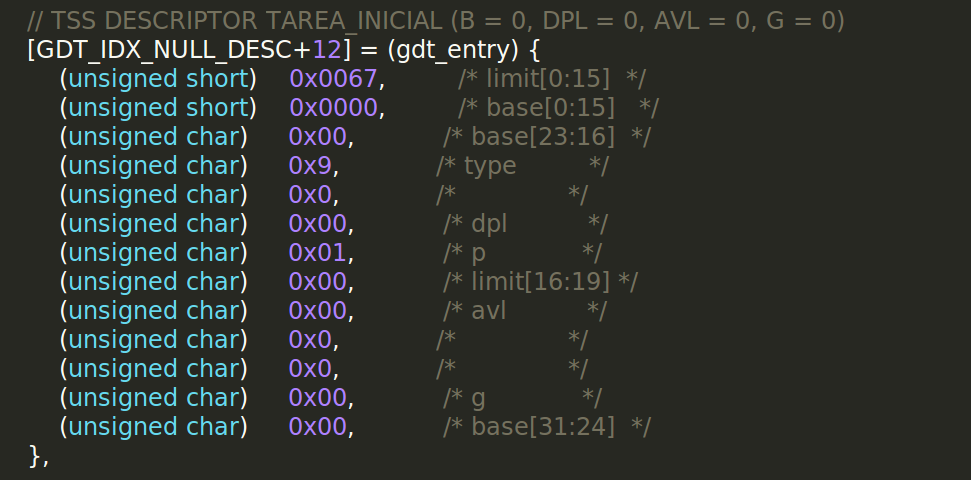
\includegraphics[width=\linewidth]{ejercicio6/gdt_tarea_inicial.png}
\caption{{\small \textit{Entrada de la \textit{GDT} correspondiente a la tarea inicial }}}
\endminipage
\end{center}
\end{figure}


Luego con la función \textit{tss\_inicializar()} le asignamos la base correspondiente.

\begin{figure}[H]
\begin{center}
\minipage{1.00\textwidth}
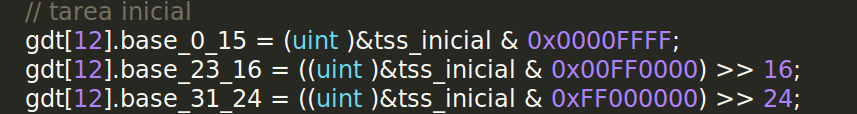
\includegraphics[width=\linewidth]{ejercicio6/tss_inicializar_base_inicial.png}
\caption{{\small \textit{Entrada de la \textit{GDT} correspondiente a la tarea inicial }}}
\endminipage
\end{center}
\end{figure}

\subsection{Ítem e): Completar la entrada de la $idle$ en la $GDT$}
Esta sección es similar a la anterior. Creamos una entrada en la \textit{GDT} para esta tarea y en la función \textit{tss\_inicializar()} seteamos los valores correspondientes para su base en la \textit{GDT} y también seteamos su TSS.\\
Como nos dicen que la tarea se encuentra en la dirección 0x00010000 ese es el valor que ponemos en la base y por el enunciado va a compartir el CR3. Lo mismo con su pila.\\

\begin{figure}[H]
\begin{center}
\minipage{1.00\textwidth}
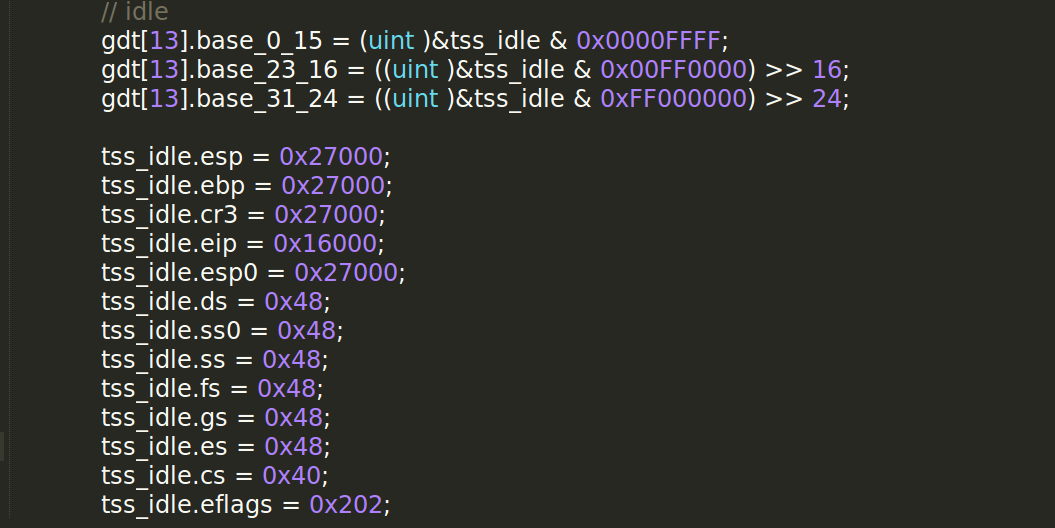
\includegraphics[width=\linewidth]{ejercicio6/tss_idle.png}
\caption{{\small \textit{Seteo la TSS de la tarea idle con los valores correspondientes}}}
\endminipage
\end{center}
\end{figure}

\subsection{Ítem f): Saltar a la tarea Idle}
Esto es simplemente hacer un jump far en el archivo kernel.asm. Como el intercambio en los valores de la TSS lo hace automáticamente el procesador simplemente agregamos al archivo \textit{kernel.asm} la siguiente linea\\
 \begin{center}
 $jmp$ 0x68:0 \\
 \end{center}

 \subsection{Ítem g): Completar la iterrución 0x46 de acuerdo al punto 4.4 del enunciado}
Para este punto lo que hacemos en la interrupción 0x46 es pushear en la pila los parametros de la interrupcion que llegan en los registros $EAX$ y $ECX$ y llamar a la función $game\_syscall\_manejar(uint syscall, uint param1)$. Lo que hace la función es, dependiendo de los parámetros que le llega, llamar a la función correspondiente para atender la interrupción las cuales pueden ser:\\

\begin{itemize}

\item $game\_perro\_mover(tarea actual, parametro 1 de la interrupcion)$.
\item $game\_perro\_cavar(tarea actual)$.
\item $game\_perro\_olfatear(tarea actual)$.
\item $game\_perro\_recibirorden(tarea actual$).

\end{itemize}

El código es el siguiente:\\


\begin{figure}[H]
\begin{center}
\minipage{1.00\textwidth}
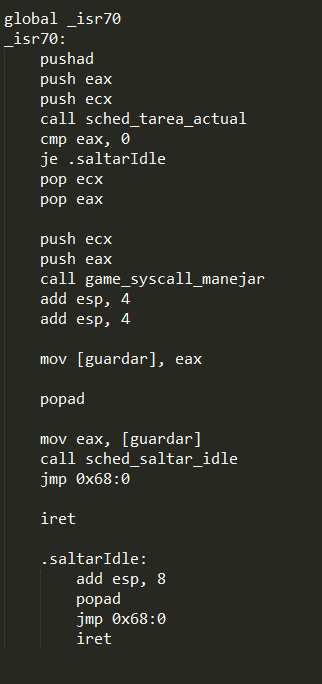
\includegraphics[width=\linewidth]{ejercicio6/isr0x46.png}
\caption{{\small \textit{Manejo de interrupciones}}}
\endminipage
\end{center}
\end{figure}

\begin{figure}[H]
\begin{center}
\minipage{1.00\textwidth}
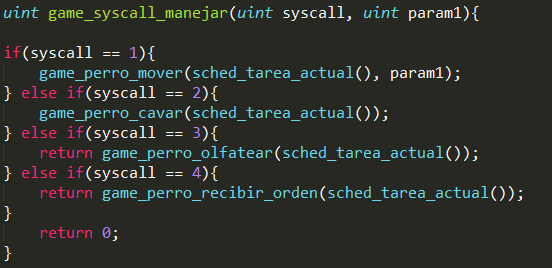
\includegraphics[width=\linewidth]{ejercicio6/syscall_manejar.png}
\caption{{\small \textit{Función que maneja los syscall}}}
\endminipage
\end{center}
\end{figure}

Notar que la imagen anterior corresponde al código final, en el cual la interrupcion, como el Tp lo pide, salta a la tarea $idle$ ,luego de haber atendido la interrupción, haciendo jmp 0x68:0. Cómo en este punto se pedía que la tarea actual no fuera desalojada, simplemente ignorar el jmp 0x68:0 

\subsection{Ítem h): Probar correr un perro}

Este itém lo testeamos y todo anduvo bien, como no va a estar en el tp final borramos el código que lo implementaba, pero fue testeado.

